\documentclass[11pt,svgnames,fleqn]{beamer}

\addtobeamertemplate{frametitle}{}
{\vspace*{0.1cm}}
\setbeamertemplate{caption}[numbered]{}

% Begin Packages
\usepackage{amsmath}
\usepackage{xspace}
\usepackage{ifthen}
\usepackage{epstopdf}
% End Packages

 
% Begin Theme
\setbeamertemplate{navigation symbols}{}
\mode<presentation>{
  \usetheme{Dresden}
  \setbeamercovered{transparent} 
}

\hypersetup{
    colorlinks=true,       % false: boxed links; true: colored links
    linkcolor=blue,        % color of internal links (change box color with linkbordercolor)
    citecolor=green,       % color of links to bibliography
    filecolor=magenta,     % color of file links
    urlcolor=blue          % color of external links
}
% End Theme

% User commands
\newcommand{\Quote}[1]{``{#1}''}
\newcommand{\Ni}{\noindent}
\newcommand{\defeq}{\stackrel{\textup{\tiny def}}{=}}
% Mathematics
\newcommand{\parn}[1]{( {#1} )}
\newcommand{\parbg}[1]{\left(  {#1} \right)}
\newcommand{\pbg}[1]{\bigl(  {#1} \bigr)}
\newcommand{\Setbg}[1]{\bigl\{ {#1} \bigr\}}
\def\Rz{\mathbb{R}}
\def\Cz{\mathbb{C}}
\def\Iz{\mathbb{N}}
\newcommand{\nliminf}[1]{\liminf\limits_{{#1} \rightarrow \infty}}
\newcommand{\nlimsup}[1]{\limsup\limits_{{#1} \rightarrow \infty}}
\newcommand{\proot}[2]{\sqrt[\leftroot{-3}\uproot{3}{#1}]{#2}}
\newcommand{\Alert}[1]{ {\Ni\color{red} {#1}}\newline }
\newcommand{\NC}[1]{{\color{red}#1}}
\newcommand{\EC}[1]{{\color{Blue}#1}}
\newcommand{\sitemize}[1]{\begin{singlespacing}\begin{itemize} {#1} \end{itemize}\end{singlespacing}}
\newcommand{\DM}[1]{\begin{displaymath} {#1} \end{displaymath}}
\newcommand{\FG}[1]{\begin{figure} {#1} \end{figure}}
\newcommand{\EX}[1]{\begin{example} {#1} \end{example}}
\newcommand{\VB}[1]{\begin{singlespacing} \verbatiminput{#1} \end{singlespacing}}
% Mathematics: ODE
\newcommand{\iode}{\protect{\makebox{$[t_0,\tend]$}}\xspace}
\newcommand{\lode}{\protect{\makebox{$[t_n,t_{n+1}]$}}\xspace}
\newcommand{\tend}{t_\text{end}}
\newcommand{\tc}[2]{(#1)_{#2}}
\newcommand{\Tp}{T}
\newcommand{\xn}{x_{n}}
\newcommand{\tn}{t_{n}}

% Author, Title, etc.

\title{Radius of Convergence}

\author{\\[1ex]
  John M. Ernsthausen
  \\[0.5ex]
  {\scriptsize Joint work with Ned Nedialkov}
}

\institute{\footnotesize
  McMaster University\\
  Canada\\
  %{\href{http:\\www.johnernsthausen.com}{\footnotesize\tt johnernsthausen.com/2018-taylor-model-workshop-talk.pdf}}\\
  \vspace*{2cm}
  \scriptsize
  Nedialkov Group Presentation\\ [0.5ex]
  October 21, 2020
}

\date{}

% The main document

\begin{document}

% Clean footer and header
\setbeamertemplate{footline}[default]
\setbeamertemplate{headline}[default]

% Title
\frame\titlepage

%%%% START DOCUMENT
\graphicspath{{images/}}

\begin{frame}{Problem}

  Given the first $k+1$ coefficients  of the  power series (PS) expansion of an  $f\,:\, \mathbb R\rightarrow\mathbb R$
\begin{align}
  f(t) =   \sum_{n=0}^{\infty} c_n (z-z_0)^n \label{eq:maineq}
\end{align}
estimate the radius of convergence (RC) of this series
 
\vspace{3mm}

We are interested in estimating the RC of Taylor series solutions of  ODEs and DAEs
\begin{itemize}
\item Needed for reliable stepsize control 
\end{itemize}



\end{frame}

%\begin{frame}{When does it converge?}
%
%  {\bf Root test}:  Let $\alpha \defeq \nlimsup{n} \proot{n}{|c_n|}$. Then
%  \begin{itemize}
%    \item[(a)] if $\alpha < 1$, then $\sum_{n=0}^{\infty} c_n$ converges;
%    \item[(b)] if $\alpha > 1$, then $\sum_{n=0}^{\infty} c_n$ diverges;
%    \item[(c)] if $\alpha = 1$, then this test gives no information.
%  \end{itemize}
%
%\vspace{2mm}
%
%  {\bf Radius of convergence (RC)}
%  Let $a_n = c_n (z - z_0)^n$. Root test $\sum_{n=0}^{\infty} a_n$
%\DM
%{
%  \nlimsup{n} \proot{n}{|a_n|} = |z-z_0| \nlimsup{n} \proot{n}{|c_n|} \defeq \tfrac{|z-z_0|}{R_c}.
%}
%Obtain
%\begin{itemize}
%  \item[(a)] if $|z-z_0| < R_c$, then the power series converges;
%  \item[(b)] if $|z-z_0| > R_c$, then the power series diverges;
%  \item[(c)] if $|z-z_0| = R_c$, then this test gives no information.
%\end{itemize}
%\end{frame}



\begin{frame}{The RC tests of CC}
{Corliss and Chang, Solving Ordinary Differential Equations 
  Using Taylor Series, ACM TOMS, 1982, pp. 114 - 144}

The coefficients of a general PS follow no patterns



  PS of a real valued function \NC{any or ODE solution?} follow a few very definite patterns
  \begin{itemize}
  \item  characterized by the
  location of primary (closest to $z_0$) singularity
  \item effects of secondary (second closest) singularities diminish as number of coefficients increases 
  \end{itemize}

\vspace{3mm}

%PS which are real valued on the real axis can have poles, logarithmic branch points, and essential singularities only on the real axis or in conjugate pairs

%\vspace{3mm}



  

\end{frame}

\begin{frame}{CC idea}
 For sufficiently large $k$, $c_k$  behave like the coefficients of
  \begin{itemize}
  \item single-pole model 
\begin{align}
 v(z) \defeq \parbg{a-z}^{-s}  \qquad s \neq 0, -1, -2, \ldots 
 \label{eq:sp}
 \end{align}
 \item or conjugate-pair model 
 \begin{align}
 w(z) \defeq \parbg{z^2 - 2 b z + a^2}^{-s} \qquad s \neq 0, -1, -2, \ldots
 \label{eq:spp}
 \end{align}
\end{itemize}

We know the coefficients of  (\ref{eq:sp}) and (\ref{eq:spp})

Find which model the $c_k$ fit, i.e. find
 $a, s$ in (\ref{eq:sp}) and $a,b,s$ if (\ref{eq:spp})

We know the RC in (\ref{eq:sp}) and (\ref{eq:spp})

Use it as an approximation of RC of (\ref{eq:maineq}).

\end{frame}

\begin{frame}{Example}
\framesubtitle{Single pole}

\end{frame}

\begin{frame}{Example}
\framesubtitle{Conjugate pair of poles}

\end{frame}
\begin{frame}

\begin{figure}
  \centering
  \vspace{-0.4cm}
  \includegraphics[width=.8\linewidth]{one-primary-pole.eps} %
  \caption{One necessarily real (primary) pole}
\end{figure}

  {\footnotesize This graph from Corliss and Chang, Solving Ordinary Differential Equations 
  Using Taylor Series, ACM TOMS, 1982, pp. 114 - 144}
\end{frame}

\begin{frame}

\begin{figure}
  \centering
  \vspace{-0.4cm}
  \includegraphics[width=.8\linewidth]{one-primary-pole-nearby-secondary-pole.eps} %
  \caption{One necessarily real (primary) pole with a secondary pole nearby}
\end{figure}

  {\footnotesize This graph from Corliss and Chang, Solving Ordinary Differential Equations 
  Using Taylor Series, ACM TOMS, 1982, pp. 114 - 144}
\end{frame}

\begin{frame}{One pole: Three term analysis}{Data fitting}

  Model the given (finite) real series (scale h) by a pole on the real axis which is radius $a$ away
  and has order of singularity $s$
  \DM
  {
    v(z) \defeq \parbg{a-z}^{-s}  \qquad s \neq 0, -1, -2, \ldots
  }
  Any function with only one primary pole or logarithmic singularity
  has the form $f(v(z))$ where $f$ is analytic in some region

  \vspace{2mm}

  On circle centered at zero $v$ has Taylor coefficients 
  \DM
  {
    k \tc{v}{k+1} = \tc{v}{k}\parbg{k+s-1}\frac{h}{a}
  }
 
  Automatic differentiation formula for $u^p$ with $p=-a$ and $u=a-z$. All derivatives of $u$ zero
  except the first one which is $-1$
\end{frame}

\begin{frame}{One pole: Three term analysis (continued)}{Data fitting}

  Derive this result from $k$ and $k-1$ recursion relations.

\vspace{2mm}

$RC \defeq a$. Then
\DM
{
  \frac{h}{RC} = \frac{h}{a} = k \frac{\tc{v}{k+1}}{\tc{v}{k}} - \parbg{k-1} \frac{\tc{v}{k}}{\tc{v}{k-1}}
}
  
  For Order $s$ (Use estimated RC from above)
\DM
{
  \text{order} \defeq s = k \frac{\tc{v}{k+1}}{\tc{v}{k}}\frac{RC}{h} - k + 1
}

  \NC{If the series has one primary pole or logarithmic singularity, this test will detect it}

  \vspace{2mm}

  Compute two estimates. Terms $N-2$, $N-1$, $N$.
  If the two estimates of $h/RC$ do not agree (Relative backward error), then series does not have
  one primary real pole or logarithmic singularity
\end{frame}

\begin{frame}{Complex conjugate pair of poles: Six term analysis}{Data fitting}

  Model the given (finite) real series (scale h) by a Complex conjugate pair of poles
  which is radius $a$ away and has order of singularity $s$

  \vspace{2mm}

  $b \in \Rz$ and $\cos \theta \defeq b/a$ (Picture would help here)

  \vspace{2mm}

  Model
  \DM
  {
    w(z) \defeq \parbg{z^2 - 2 b z + a^2}^{-s} \qquad s \neq 0, -1, -2, \ldots
  }

  \vspace{2mm}

  On circle centered at zero $w$ has Taylor coefficients 
  \DM
  {
    k \tc{w}{k+1} = 2 \tc{w}{k}\parbg{k+s-1}\frac{h}{a} \cos \theta 
    - \tc{w}{k-1}\parbg{k+2s-2}\parbg{\frac{h}{a}}^2
  }
 
  Reduced derivative formula for $u^p$ with $p=-a$ and $u=z^2 - 2 b z + a^2$.
\end{frame}

\begin{frame}{Six term analysis (continued)}{Data fitting}

 Unknowns:
  $\beta_1 = (h/a) \cos \theta$,
  $\beta_2 = s \beta_1$,
  $\beta_3 = (h/a)^2$,
  $\beta_4 = s \beta_3$

  \vspace{2mm}

  Equations:
  \begin{align*}
    k \tc{w}{k+1} & = \parbg{k-1} \tc{w}{k} \beta_1 +  \tc{w}{k} \beta_2 \\
                  & - \parbg{k-2} \tc{w}{k-1} \beta_3 - 2 \tc{w}{k-1} \beta_4
  \end{align*}
  for $k=N-1, N-2, N-3, N-4$

  \vspace{2mm}

  Linear system. Feasible solution unless $\beta_3 < 0$ or $|\cos \theta| > 1$ or
  large residual where residual is backward error checked against
  data from $N-5$ equation

  \vspace{2mm}

  Two values for $s$ may disagree (a lot).
  Optimization problem minimizing norm of $\beta$.
  Enforce $\beta_3 \geq 0$ and $|\cos \theta| \leq 1$ in box constraints.

\end{frame}

\begin{frame}{Top line analysis: The ratio test}{Data fitting}

Best linear fit $y(k) = m k + b$ in the $2$-norm to the points
\DM
{
  \Setbg{(n, \log_{10} | c_{n} |), (n+1, \log_{10} |c_{n+1}|), \ldots, (N, \log_{10} |c_{N}|)}
}
for some sufficiently large $n$ so that convergence guaranteed
\vspace{4mm}

$\sum_{n=0}^{\infty} c_n$ converges then $c_n \rightarrow 0$ as $n \rightarrow \infty$
\NC{The model parameter $m$ will be negative}

\vspace{4mm}

Compute the ratio in the ratio test with linear least squares best fit model. Then
\DM
{
  \log_{10} \left| \tfrac{y(k+1)}{y(k)} \right| = \log_{10} | y(k+1) | - \log_{10} | y(k) | = m
}
which is independent of $k$.

\end{frame}

\begin{frame}{Top line analysis (continued)}{Data fitting}

Have convergence analysis for top-line analysis

\vspace{4mm}

To find Order of singularity $\mu$ and the best possible $RC$

  \begin{itemize}

    \item Integrate sequence 3 times. Set $\mu = 4$

    \vspace{4mm}
  
    \item Search for the sequence which opens downward.
      
    \vspace{4mm}
      
    \item Differentiate the result up to 7 times reducing $\mu$ by one for each differentiation

    \vspace{4mm}

    \item If cannot find such a sequence, conservatively use the final estimate $RC$ but $\mu$ unknown
  \end{itemize}
\end{frame}

\begin{frame}

\begin{figure}
  \centering
  \vspace{-0.4cm}
  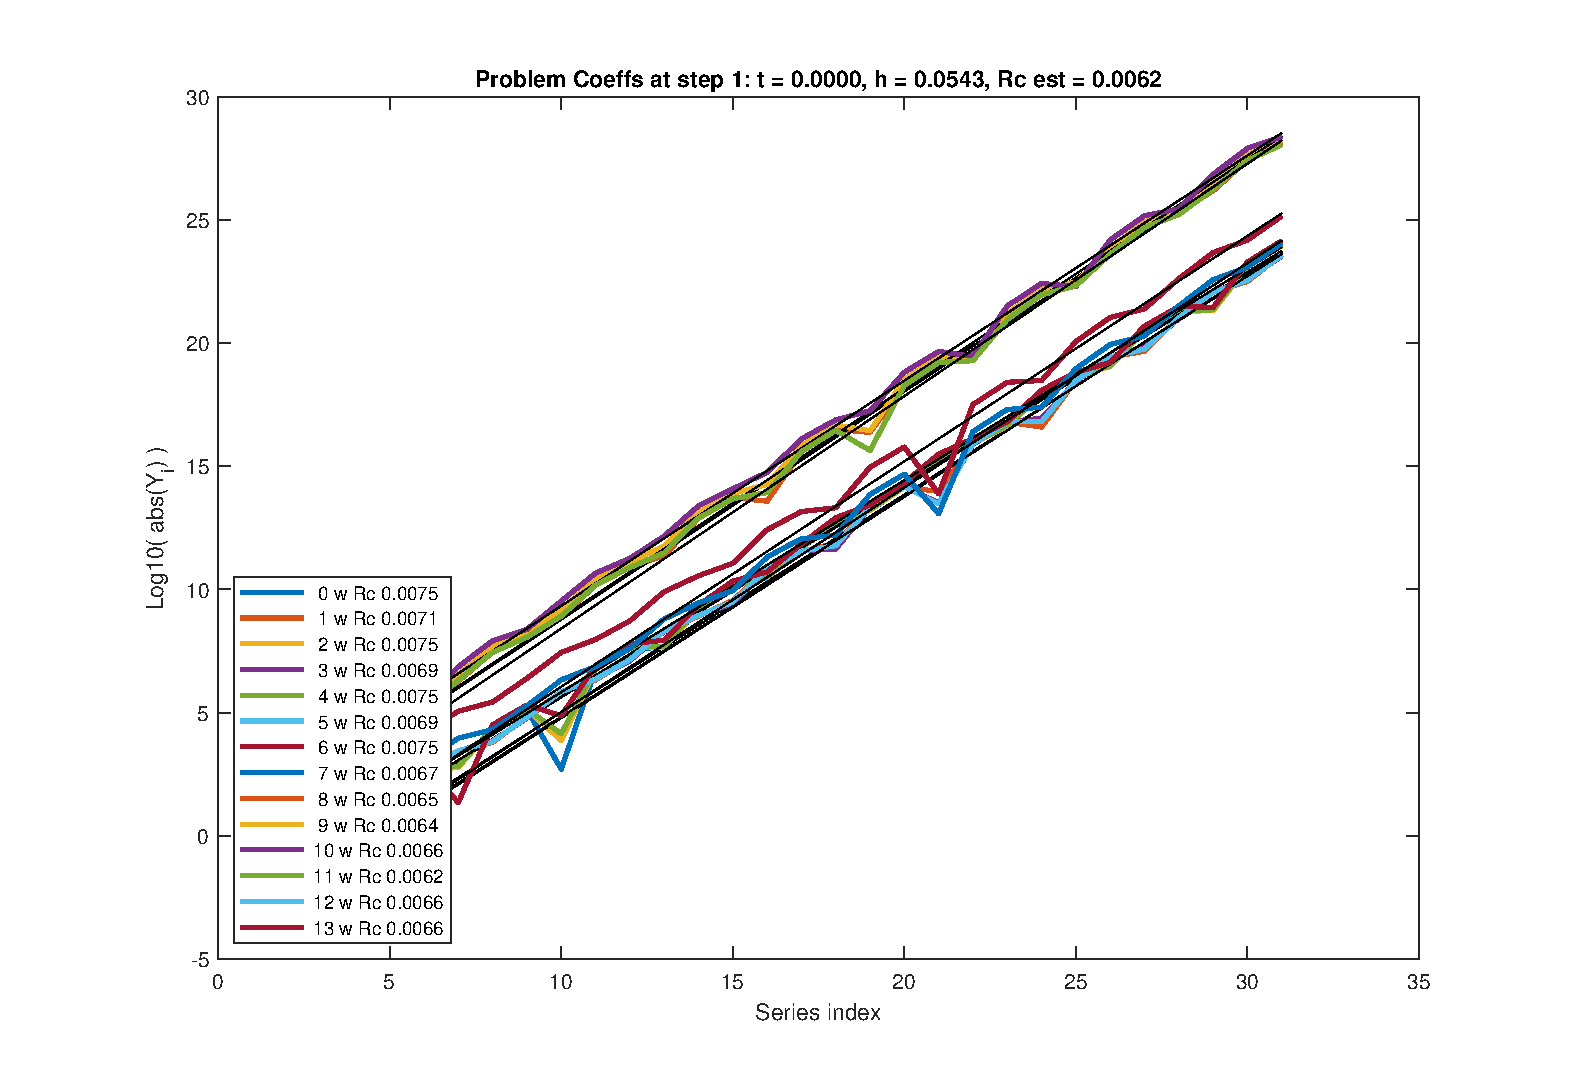
\includegraphics[width=.9\linewidth]{divergent.eps} %
  \caption{Top-line analysis shows divergent TS and rejected step}
\end{figure}

\end{frame}

\begin{frame}

\begin{figure}
  \centering
  \vspace{-0.4cm}
  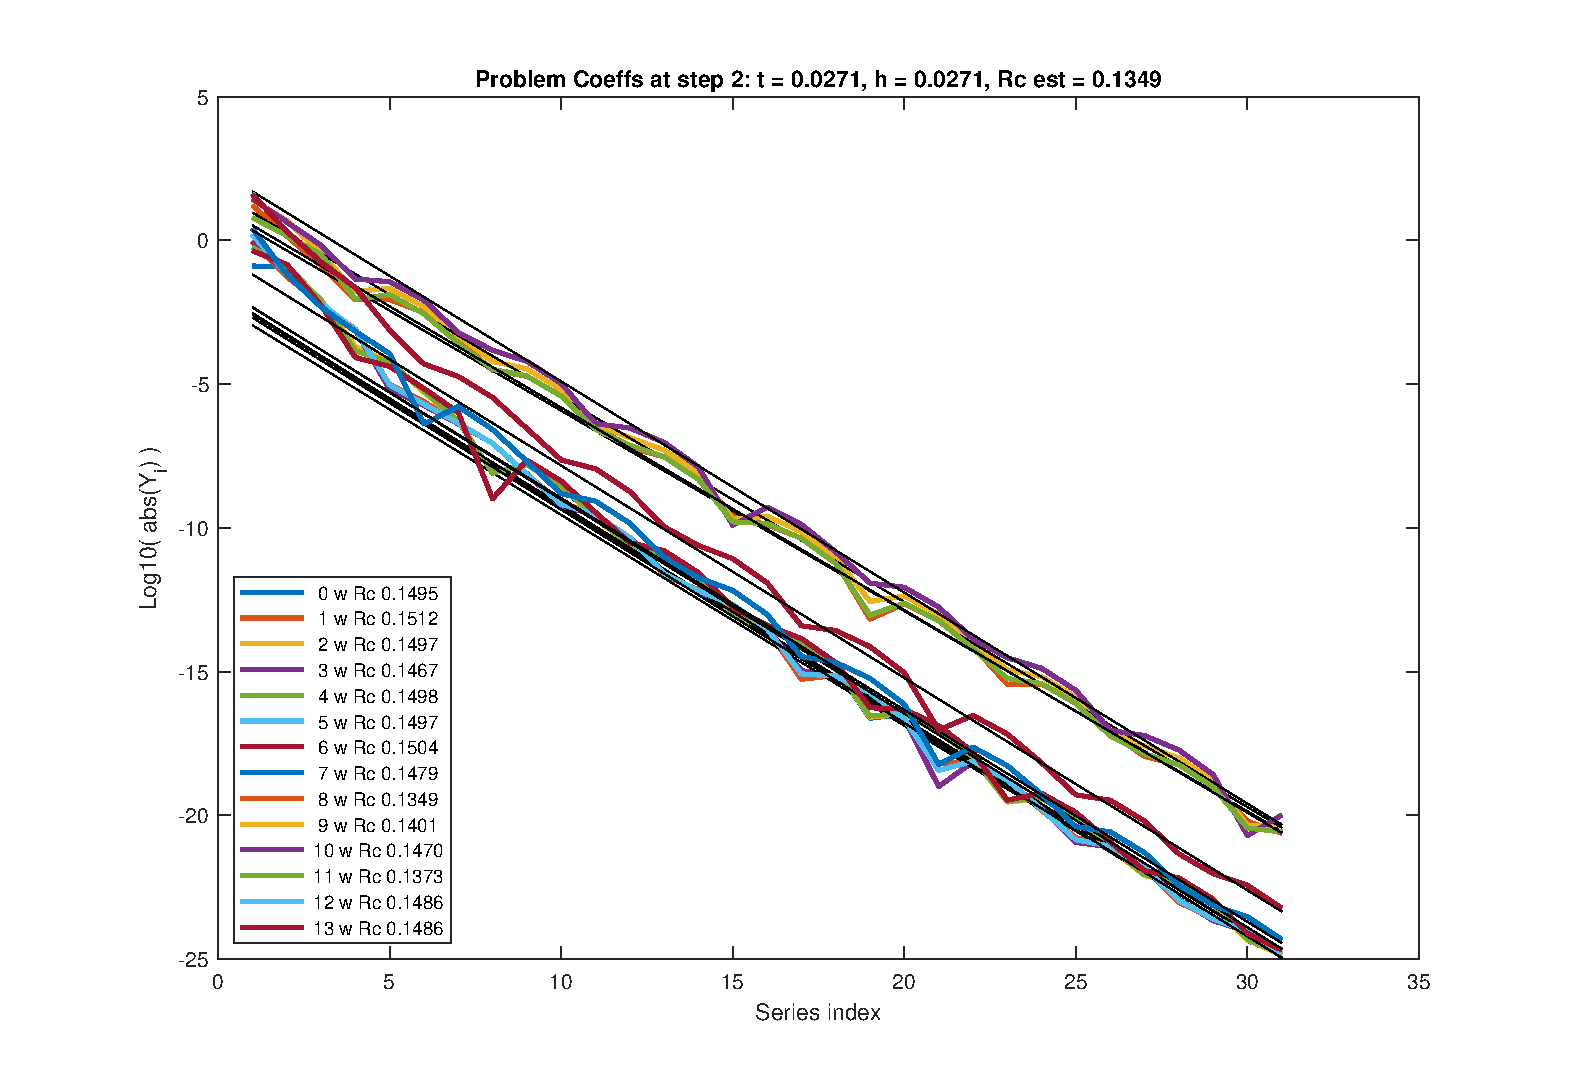
\includegraphics[width=.9\linewidth]{convergent.eps} %
  \caption{Top-line analysis indicates convergent TS and stepsize}
\end{figure}

\end{frame}

\end{document}
